\problem{Problème II: Modèle de Hubbard}
\blindduck{num1}

\begin{figure}[h!]
    \begin{center}
        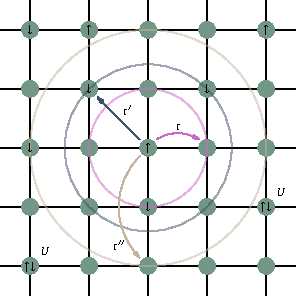
\includegraphics[width=0.5\textwidth]{../figs/2d_lattice.pdf}
    \end{center}
    \caption{Caption. Caption captioncaptioncaption? Caption caption.}
    \label{fig: fig_num_2}
\end{figure}

\blindduck

\begin{align}
    \boxed{
        d = ra^k e.
    }
    \label{eq: test_2}
\end{align}

\clearpage
